\documentclass[ruled,graybox]{svmult}
%\usepackage{mathptmx}        % selects Times Roman as basic font
%\usepackage{helvet}          % selects Helvetica as sans-serif font
%\usepackage{courier}         % selects Courier as typewriter font

%\usepackage[document]{ragged2e}

\usepackage{chapterbib}


\usepackage{graphicx,color}
\usepackage{amsmath, amssymb}
\usepackage[ruled]{algorithm}
\usepackage{algorithmic}
\usepackage{url}
\usepackage{subcaption}
\usepackage{booktabs}
\usepackage{diagbox}
\usepackage{bm}
\usepackage{tabularx}

% TODO marker
\usepackage{color}
\usepackage{xspace}
\definecolor{ScarletRed}{rgb}{0.80,0.00,0.00}
\newcommand\todo[1]{\textcolor{ScarletRed}{\textbf{\colorbox{yellow}{\small TODO:}} [\emph{#1}]}\xspace}

\setcounter{secnumdepth}{3}

\usepackage{enumitem}
\usepackage{bm}
\usepackage{relsize}
\usepackage{listings}



\frontmatter
\mainmatter
\backmatter


\begin{document}



\frontmatter%%%%%%%%%%%%%%%%%%%%%%%%%%%%%%%%%%%%%%%%%%%%%%%%%%%%%%
%\include{dedic}


\thispagestyle{empty}
\providecommand\pdfbookmark[3][]{} \pdfbookmark[0]{Title Page}{bm:Title}
\vspace*{1cm}
\vfill
\begin{center}
\textsc{\huge{Introduction to Computational Intelligence}}\\
\vfill
Editors\\[\baselineskip]
\textsc{\Large{Leandro L. Minku, George Cabral, Marcella Martins, Markus Wagner}}
\vfill
\end{center}
\begin{figure}[ht!]
\centering

\includegraphics[height=1.5cm]{ieee-logo.png}
\hspace{0.5cm}

\includegraphics[height=1.5cm]{ieee-cis-logo.jpg}
\end{figure}
\begin{center}
% Cold Atoms Research Group\\[-0.8em]
An IEEE Computational Intelligence Society Open Book\\
DOI: 10.5281/zenodo.7537827\\[-0.8em]
\end{center}
%\copyright\ Copyright by \MakeUppercase{\@Author},~\@Year\\
%All Rights Reserved
\clearpage


%%%%%%%%%%%%%%%%%%%%%%foreword.tex%%%%%%%%%%%%%%%%%%%%%%%%%%%
% sample foreword
%
% Use this file as a template for your own input.
%
%%%%%%%%%%%%%%%%%%%%%%%% Springer %%%%%%%%%%%%%%%%%%%%%%%%%%

\preface

Due to its power to solve large scale problems and analyse vast amounts of data that would be difficult or time consuming for humans to deal with manually, the field of Computational Intelligence has grown tremendously in importance over the past years. We nowadays see widespread use of computational intelligence in the most varied applications. A few examples include approaches to detect credit card fraud, recognise faces, transcribe voice to text, identify spam, route and schedule deliveries, design aerodynamic high speed trains, etc. 

It is thus not surprising that we see a growing number of people who are keen to learn about this field. However, there is a lack of open resources that combine several different types of computational intelligence approaches in one place, so that people can easily get an introduction to this field. Those eager to learn about computational intelligence may also struggle to get help from others when trying to understand existing approaches, whereas those willing to start teaching this topic may struggle to find free resources to guide them. 

This \textit{open} book has been created as a community effort to overcome these issues. The notion of \textit{openness} of this book includes, but goes beyond open access. In addition to being available through an open license so that resources on computational intelligence are accessible to all, this book is hosted in github at:

\

\noindent \url{https://github.com/ieee-cis/IEEE-CIS-Open-Access-Book-Volume-1}. 

\

Such initiative will enable the book to be continuously improved over time through pull requests to fix typos, add clarifications, add new exercises, add examples of open software code, add video lectures on the content, etc. Therefore, this book is \textit{open} for the community to propose enhancements over time. The book is also associated to github discussion boards, so that people can ask questions and the community can help with answering those questions, creating an \textit{open} community that all can join in. 

If you would like to propose an enhancement through a pull request to this book, we ask you to first contact the current chair of the IEEE Computational Intelligence Society Education Portal Subcommittee (\url{https://cis.ieee.org/}). The chair will advise you on how to proceed. Minor changes to existing chapters will be handled by the subcommittee directly, whereas the subcommittee will liaise with the original authors to obtain their consent for incorporating larger pull requests. 

We thank all the authors who have contributed chapters to this book, all the anonymous reviewers who have reviewed the chapters, and all the community members who will contribute with this book and discussion boards in the future.

We hope that you will find the book a useful resource to learn about computational intelligence.

\vspace{\baselineskip}
\begin{flushright}\noindent
Leandro L. Minku, on behalf of the editors of the\\
IEEE CIS Computational Intelligence Open Book -- First Edition 
\end{flushright}



\abouteditors

\begin{center}
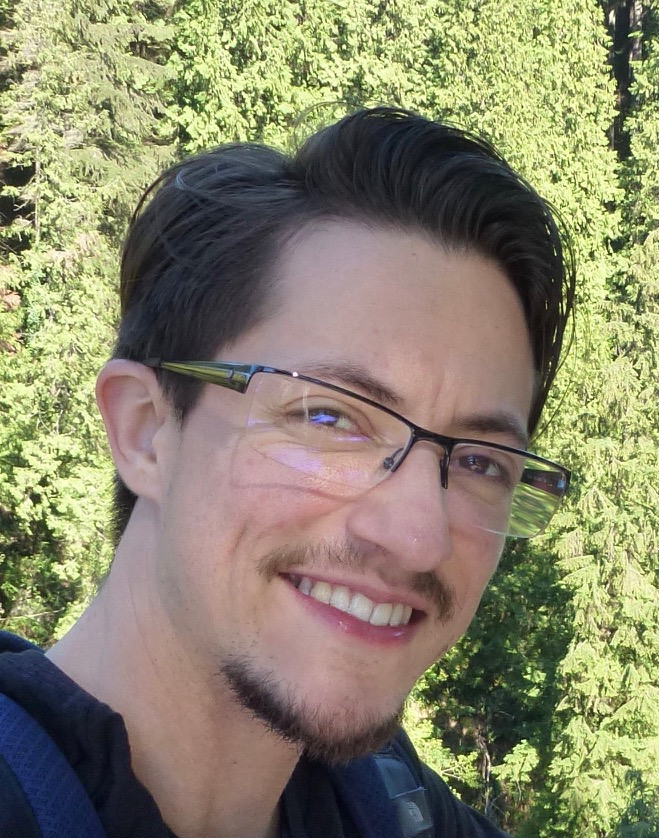
\includegraphics[width=.3\textwidth]{Photos/minku.jpg}
\end{center}

Dr. Leandro L. Minku is an Associate Professor at the School of Computer Science, University of Birmingham (UK). Prior to that, he was a Lecturer in Computer Science at the University of Leicester (UK). He received the PhD degree in Computer Science from the University of Birmingham (UK) in 2010. Dr. Minku's main research interests are machine learning in non-stationary environments / data stream mining, online class imbalance learning, ensembles of learning machines and computational intelligence for software engineering. His work has been published in internationally renowned journals such as IEEE Transactions on Neural Networks and Learning Systems, IEEE Transactions on Knowledge and Data Engineering, IEEE Transactions on Software Engineering and ACM Transactions on Software Engineering and Methodology. Among other roles, Dr. Minku is Associate Editor-in-Chief for Neurocomputing, Senior Editor for IEEE Transactions on Neural Networks and Learning Systems, and Associate Editor for Empirical Software Engineering Journal and Journal of Systems and Software. He was also the General Chair for the International Conference on Predictive Models and Data Analytics in Software Engineering (PROMISE 2019 and 2020), and Co-chair for the Artifacts Evaluation Track of the International Conference on Software Engineering (ICSE 2020).

\begin{center}
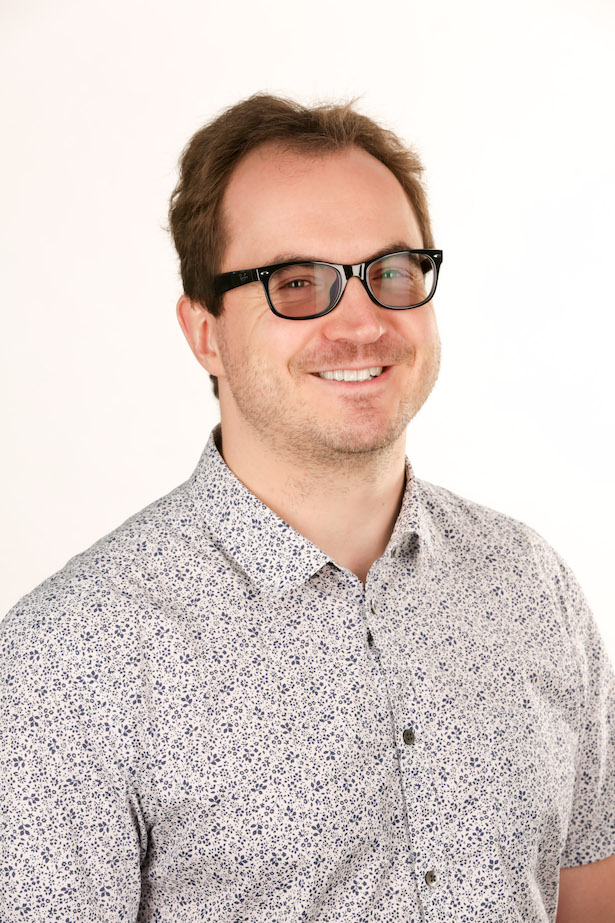
\includegraphics[width=.3\textwidth]{Photos/wagner.jpg}
\end{center}

Dr. Markus Wagner is an Associate Professor at Faculty of Information Technology, Monash University (Australia). He has done his PhD studies at the Max Planck Institute for Informatics in Saarbruecken, Germany and at the University of Adelaide, Australia. For the outcomes of his studies, he has received the university's Doctoral Research Medal --- the first for his school --- and three best paper awards. His research topics range from mathematical runtime analysis of heuristic optimisation algorithms and theory-guided algorithm design to applications of heuristic methods to renewable energy production, professional team cycling and software engineering. So far, he has been a program committee member 80+ times, and he has written 150+ articles with 200+ different co-authors. He has chaired several education-related committees within the IEEE CIS, where he also served as founding chair of two task forces. Markus is an ACM Lifetime Member, is on SIGEVO's Executive Board and serves as the first ever Sustainability Officer. He has contributed to GECCOs as Workshop Chair and Competition Chair, and most recently as General Chair.


\begin{center}
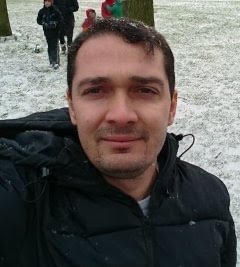
\includegraphics[width=.3\textwidth]{Photos/cabral.jpg}
\end{center}

Dr. George Cabral received his PhD degree from the Federal University of Pernambuco (Brazil) in 2014. His postdoc was conducted at the University of Birmingham (UK) in 2019. Currently, he is an adjunct professor at the Department of Computing at the Federal Rural University of Pernambuco (Brazil). He serves as reviewer for reputed journals such as Neurocomputing and Applied Software Computing. In addition, he has systematically served as committee member in prestigious conferences such as ICSE, ASE and ICONIP. His recent plublications include papers in reputed venues such as IEEE Transactions on Software Engineering and at the International Conference on Software Engineering (ICSE). He has taught courses involving Computational Intelligence for more than a decade and since 2020 he is applying this knowledge in practice for auditing public finances at the state of Pernambuco - Brazil. His research interests include Novelty Detection, One-class Classification, Data Mining, Class Imbalance Learning, Software Defect Prediction, Concept Drift, Online Learning, etc.


\contributors

The list below contains information about contributors who have made large revisions to chapters of this book.

\begin{tabularx}{1.2\textwidth}{|l|l|X|} \hline
Contributor & Chapter & Commit \\ \hline
Leandro L. Minku & Chapter \ref{chp:into-learning-systems} & \url{https://github.com/ieee-cis/IEEE-CIS-Open-Access-Book-Volume-1/commit/186ef1d4c1c2b47047981f7cbb8dc8d05dd80651} \\ \hline
\end{tabularx}

%\include{acknow}

\tableofcontents
\listoffigures
\listoftables

\notation

In general, the following mathematical notations will be used in this book:

\begin{itemize}
\item Scalar: lower case, e.g., $a$, $b$.
\item Column vector: lower case, bold, e.g., $\textbf{x}$.
\item Vector element: lower case with subscript, e.g., $x_1$, $x_2$.
\item If enumerating vectors (e.g., having multiple vectors), superscript will be used to differentiate this from indices, e.g., $\textbf{x}^{(1)}$, $\textbf{x}^{(2)}$.
\item Matrix: upper case, bold, e.g., $\textbf{X}$.
\item Matrix element: upper case with subscripts, e.g., $X_{1,2}$.
\item When considering that a matrix is a vector of vectors, row $i$ and column $j$ can be represented by $\textbf{x}^{(i)}_j$.
\item Sets: calligraphy font in upper case, e.g., $\mathcal{T}$.
\item Generic data structure with unspecified format (e.g., it could be a vector, a matrix, or any other structure): lower case, bold, e.g., $\textbf{x}$.
\end{itemize}

\mainmatter%%%%%%%%%%%%%%%%%%%%%%%%%%%%%%%%%%%%%%%%%%%%%%%%%%%%%%%
\include{"Part 1 - History and Definitions/History and Definitions"}
\include{"Part 1 - History and Definitions/Introduction"}


\include{"Part 2 - Search-Based Optimization/Introduction/Search-Based Optimization"}
\include{"Part 2 - Search-Based Optimization/Local Search/Local Search"}
\include{"Part 2 - Search-Based Optimization/Simulated Annealing/Simulated Annealing"}
\include{"Part 2 - Search-Based Optimization/Particle Swarm Optimization/Particle Swarm Optimization"}
\include{"Part 2 - Search-Based Optimization/Other Search-Based Optimization Approaches/Other Search-Based Optimization Approaches"}

\include{"Part 3 - Learning Systems/Introduction/Learning Systems"}

\begin{flushright}
\Large\textbf{\partname\ \thepart -(A)}\\
\Large\textbf{Supervised Learning}
\end{flushright}
\addcontentsline{toc}{part}{\partname\ \thepart -(A) Supervised Learning}

\include{"Part 3 - Learning Systems/Supervised Learning/k-Nearest Neighbors/k-Nearest Neighbors"}
\include{"Part 3 - Learning Systems/Supervised Learning/Multilayer Perceptron/Multilayer Perceptron"}
\include{"Part 3 - Learning Systems/Supervised Learning/Deep Learning/Deep Learning"}
\include{"Part 3 - Learning Systems/Supervised Learning/Naive Bayes/Naive Bayes"}
\include{"Part 3 - Learning Systems/Supervised Learning/Evaluation Unsupervised/Evaluation Unsupervised"}

\begin{flushright}
\Large\textbf{\partname\ \thepart -(B)}\\
\Large\textbf{Unsupervised Learning}
\end{flushright}
\addcontentsline{toc}{part}{\partname\ \thepart -(B) Unsupervised Learning}

\include{"Part 3 - Learning Systems/Unsupervised Learning/k-Means/k-Means"}
\include{"Part 3 - Learning Systems/Unsupervised Learning/Hierarchical Clustering/Hierarchical Clustering"}
\include{"Part 3 - Learning Systems/Unsupervised Learning/DBScan/DBScan"}
\include{"Part 3 - Learning Systems/Unsupervised Learning/Expectation-Maximization/Expectation-Maximization"}
\include{"Part 3 - Learning Systems/Unsupervised Learning/Self-Organizing Maps/Self-Organizing Maps"}
\include{"Part 3 - Learning Systems/Unsupervised Learning/Evaluation/Evaluation"}



\backmatter%%%%%%%%%%%%%%%%%%%%%%%%%%%%%%%%%%%%%%%%%%%%%%%%%%%%%%%



\end{document}
